\chapter{\label{Intro}Introduction}

The rendering problem of calculating the radiance(brightness) of surfaces in 3D scene is very important in 3D computer graphics. Given a geometrical location and optical characteristics(reflectivity) of surfaces along with light sources in 3D scene our concern is to calculate radiance and generate realistic image of scene illuminated with light source.

\section{Direct and Indirect illumination}
Global illumination or indirect illumination is a name for a group of algorithms used in 3D computer graphics that are meant to add more realistic lighting to 3D scenes. Such algorithms take into account not only the light which comes directly from a light source (direct illumination), but also light rays from the same source which are reflected by other surfaces in the scene(indirect illumination).
As a result indirect lighting realistic features like light bouncing and color bleeding(between pair of adjacent surfaces) is also achieved in the process.

A well known global illumination algorithm is ray-tracing \cite{Whitted} in which computes  radiance of the area of the surface of the scene
seen from one given viewpoint. In other words it only calculates radiance of the points which are visible in final image. Thus for different viewpoint we need to run algorithm again, making it viewpoint dependent.

Radiosity algorithms are set of global illumination algorithms calculating radiance of surfaces reflecting light diffusely(equal energy in all the directions above the surface)[Gallagar]. In other words radiosity takes the 3D scenes with Lambertian surfaces as a input. Opposite to ray-tracing, radiosity calculates radiance of all the surfaces in the scene. This allows the computation to be viewpoint independent i.e. solution of problem can be used to generate images of scene from arbitrary viewpoint. The solution of the problem is radiosity function over the domain of surfaces in the scene.

Radiosity algorithms were first developed in about 1950 in the engineering field of heat transfer. They were later refined specifically for the problem of rendering 3D computer graphics by Goral et al.\cite{Goral}. Goral et al. approximated the radiosity function as piecewise constant function over the domain of surfaces in the scene.In other words surfaces are divided in to discrete areas({\em elements}) over which radiance is assumed to be constant. Law of conservation of energy give rise to n linear equation with n unknowns. The system of linear equations is solved to find the solution. The algorithm requires the calculation interaction coefficient between ordered pair of elements. Thus $n^2$ interaction coefficients has to be calculated. This algorithm results in blocky images of the scene. To get realistic looking images, smoothening filters are used to remove blockiness. 
\begin{figure}[tbh]
\centering{}
\captionsetup{justification=centering}
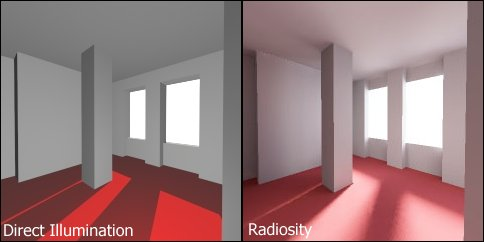
\includegraphics[width=5in]{DirectIndirect.jpg}
\caption{\label{fig:directindirect}Difference between direct illumination and radiosity(indirect illumination)}
\end{figure}
Figure \ref{directindirect} shows an example of difference between direct and indirect illumination. The image on the left in the figure is rendered with standard direct illumination renderer. It consist of mainly two lighting effects {\bf decide whether two lighting efect or 3 as in wikipedia}
Kajia [Kajia] proposed radiosity integral equation, a Fredholm integral equation of the $2^{nd}$ kind. { \bf Radiosity integral equation is described in sectoion 2 in detail.} Method proposed by Goral et al. \cite{Goral} is approximation to radiosity integral equation. Thus by describing  our radiosity problem in the form of integral equation [CAS][llmw][qlmw][haar] we can exploit various methods to solve the problem. For example  {\bf give and explain some papers on solving Fredholm IE and Galerking algorithm}. In general this algorithms proceeds in two parts. First part is to project the problem into finite dimensional basis to approximate the problem as system of linear equation. Second part calculates the solution of the linear equation and calculates the approximate solution of the problem{\bf  finite linear combination of the basis vectors in  $V_n$ }. Thus selection of finite dimensional space and basis{\bf explain this space and basis} is crucial for increasing the accuracy of the problem.

Similar approach was taken by et al. [hanarahan] and projected radiosity integral equation to finite dimensional function space. In particular he used space of piecewise linear function. Zatz [Zatz] has used Legendre polynomials as basis of finite dimensional space and solved the radiosity integral equation. One can use wavelet basis for given finite dimensional space. Since wavelets,due to its vanishing moments, are very good at approximating the smooth function with less number of coefficients. Thus projecting the radiosity problem into wavelet basis will give sparse system of linear equations. This results in the faster computation in second part of the Galerkin algorithm. 

{\bf The idea of wavelet radiosity is essentially to employ a Galerkin approach where basis functions are chosen to be wavelets with vanishing moments. The discrete system generated by the Galerkin method is generally a blockwise sparse sys-:
tern of linear equations, Mx = b. Using wavelet basis functions with the vanishing moment
property results in numerous elements of the matrix M being very small. Wavelet radiosity
follows the general method for the solution of integral equations presented by [beyl91] and
exploits this property in two ways:
Small kernel coefficients are set to zero, with the remaining system being:sparse. This
allows for a fast solution method} Beylkin et al. [3] made the observation that integral operators satisfying very general smoothness conditions can be approximated to any finite precision with only O(n) coefficients
when projected into a wavelet basis instead of the usual O($n^2$).
This remarkable result means that, in practice, integral equations
governed by smooth kernels lead to sparse matrices that can be
solved in linear time. Since the radiosity kernel is, in general,
a smooth function of the type required by this theorem, wavelet
methods can be used to obtain O(n) complexity radiosity algo-
rithms.Gortler et al. [Gortler] used wavelet basis for projection into finite dimensional space and call this set of algorithms as {\em wavelet radiosity} [schr96][chri94]. \\\\
\section{Organization of the Report}
{\bf Describe the sections}